%%%%%%%%%%%%%%%%%%%%%%%%%%%%%%%%%%%%%%%%%
% baposter Landscape Poster
% LaTeX Template
% Version 1.0 (11/06/13)
%
% baposter Class Created by:
% Brian Amberg (baposter@brian-amberg.de)
%
% This template has been downloaded from:
% http://www.LaTeXTemplates.com
%
% License:
% CC BY-NC-SA 3.0 (http://creativecommons.org/licenses/by-nc-sa/3.0/)
%
%%%%%%%%%%%%%%%%%%%%%%%%%%%%%%%%%%%%%%%%%

%----------------------------------------------------------------------------------------
%	PACKAGES AND OTHER DOCUMENT CONFIGURATIONS
%----------------------------------------------------------------------------------------

\documentclass[landscape,a0paper,fontscale=0.3]{baposter} % Adjust the font scale/size here

\usepackage{float} % Required for multiple columns
\usepackage{placeins}
\usepackage{stfloats}
\usepackage[utf8]{inputenc}
\usepackage[T1]{fontenc}
\usepackage[english]{babel}

\usepackage{tabu}
\usepackage{tabularx}
\usepackage{booktabs, hhline}
\usepackage{subfig}
\usepackage{graphicx} % Required for including images
\graphicspath{{figures/}} % Directory in which figures are stored
\usepackage{graphicx}
\usepackage{amsmath} % For typesetting math
\usepackage{amssymb} % Adds new symbols to be used in math mode

\usepackage{booktabs} % Top and bottom rules for tables
\usepackage{enumitem} % Used to reduce itemize/enumerate spacing
\usepackage{palatino} % Use the Palatino font
\usepackage[font=small,labelfont=bf]{caption} % Required for specifying captions to tables and figures

\usepackage{multicol} % Required for multiple columns
\setlength{\columnsep}{1.5em} % Slightly increase the space between columns
\setlength{\columnseprule}{0mm} % No horizontal rule between columns
\selectcolormodel{cmyk}

\usepackage{tikz} % Required for flow chart
\usetikzlibrary{shapes,arrows} % Tikz libraries required for the flow chart in the template

\newcommand{\compresslist}{ % Define a command to reduce spacing within itemize/enumerate environments, this is used right after \begin{itemize} or \begin{enumerate}
\setlength{\itemsep}{1pt}
\setlength{\parskip}{0pt}
\setlength{\parsep}{0pt}
}

\definecolor{darkgreen}{cmyk}{0.2394,0.0000,0.2394,0.2627}
\definecolor{orange}{cmyk}{0.0000,0.7294,1.0000,0.0000} 
\definecolor{floralwhite}{cmyk}{0.0000,0.0196,0.0588,0.0000}
\definecolor{gray}{cmyk}{0.0000,0.0000,0.0000,0.0392}
\definecolor{lightgreen}{cmyk}{0.7554,0.0000,0.7554,0.4549}
\definecolor{lightblue}{rgb}{0.145,0.6666,1} % Defines the color used for content box headers

\begin{document}

\begin{poster}
{
headerborder=closed, % Adds a border around the header of content boxes
colspacing=1em, % Column spacing
bgColorOne=white, % Background color for the gradient on the left side of the poster
bgColorTwo=white, % Background color for the gradient on the right side of the poster
borderColor=lightblue, % Border color
headerColorOne=lightblue, % Background color for the header in the content boxes (left side)
headerColorTwo=green, % Background color for the header in the content boxes (right side)
headerFontColor=black, % Text color for the header text in the content boxes
boxColorOne=white, % Background color of the content boxes
textborder=roundedleft, % Format of the border around content boxes, can be: none, bars, coils, triangles, rectangle, rounded, roundedsmall, roundedright or faded
eyecatcher=true, % Set to false for ignoring the left logo in the title and move the title left
headerheight=0.1\textheight, % Height of the header
headershape=roundedright, % Specify the rounded corner in the content box headers, can be: rectangle, small-rounded, roundedright, roundedleft or rounded
headerfont=\Large\bf\textsc, % Large, bold and sans serif font in the headers of content boxes
%textfont={\setlength{\parindent}{1.5em}}, % Uncomment for paragraph indentation
linewidth=2pt % Width of the border lines around content boxes
}
%----------------------------------------------------------------------------------------
%	TITLE SECTION 
%----------------------------------------------------------------------------------------
%
{
\includegraphics[height=5em]{irit.png}} % First university/lab logo on the left
%
{\bf\LARGE\ \textsc{Guarnary}: Mitigating Buffer Overflow Using Hardware Assisted Virtualization Features} % Poster title \vspace{0.2em}
{\textsl{\small Stella Bitchebe$^{+,o}$, Yves KONE$^{+,*}$, Alain Tchana$^{+}$, $^{+}$Labo LIP - Ecole Normale Sup\'erieure de Lyon, $^{o}$Labo I3S - Université Côte d'Azur, $^{*}$Labo IRIT - INP Toulouse}\\ \vspace{0.2em}

\includegraphics[height=2em]{I3S.png}
\hspace*{6em}

\includegraphics[width=0.15\linewidth]{compas.png}
\hspace*{6.3em}

\includegraphics[scale=.2]{enslogo.png}}
{
\includegraphics[height=5em]{logo_lip_HD.png}} 

%----------------------------------------------------------------------------------------
%	CTX & MOTIV
%----------------------------------------------------------------------------------------

\headerbox{1. Context and Motivation}{name=ctxmotiv,column=0,span=2}
{
    \begin{itemize}
        \item Buffer overflow is the top one vulnerability in 2021 according to the CWE (Common Weakness Enumeration)~\cite{top25}
        \item Secure Allocators (Slimguard~\cite{slimguard}, Guarder~\cite{guarder}, etc.) use \emph{guardians} to prevent and detect overflows
        \item Existing types of guardians: 
            \begin{itemize}
                \item \textcolor{blue}{\bf Canary}: Low memory overhead + Asynchronous detection
                \item \textcolor{blue}{\textbf{Guard Page}}: High memory overhead + Synchronous detection
            \end{itemize}
    \end{itemize}

    \centering
    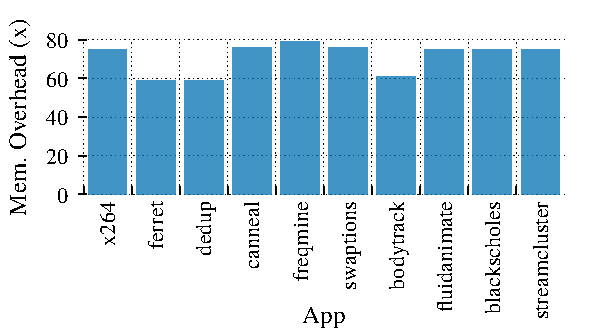
\includegraphics[width=.4\columnwidth]{figures/waste1}
    \captionof{figure}{Memory waste of PARSEC when all application's buffers are allocated at the boundary of a guard page using Slimguard as the memory allocator.}
%\vspace{-4cm} % When there are two boxes, some whitespace may need to be added if the one on the right has more content
}


\headerbox{2. Dilemma: Synchronuous Dectection vs. Memory Overhead}{name=dilem, column=2, span=2}
{
    \begin{multicols}{2}
        \begin{itemize}
            \item \textcolor{blue}{Security distance}: for a vulnerable buffer \texttt{b}, it is the number of bytes that separate it from a guardian
            \item \textcolor{blue}{Protection frequency}: \texttt{F} is called the protection frequency if a guard page is placed for every \texttt{F} allocated buffers
            \item User configures \texttt{F} and the allocator combines guard pages with canaries to minimize the security distance while optimizing the memory consumption
        \end{itemize}

        \vspace{0.2cm}

        \centering
        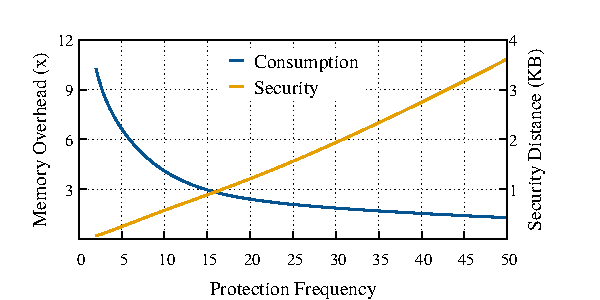
\includegraphics[width=.65\columnwidth]{figures/blackscholes}
        \captionof{figure}{Memory waste and average security distances of PARSEC-\texttt{blackscholes} when varying the protection frequency.}
        \vspace*{5mm}
        \begin{minipage}{\columnwidth}
            \centering
            \resizebox{\columnwidth}{!}
            {%
            \begin{tabular}{l l l l l l l l l l l }
                \toprule\hline
                Frequency & 1 & 2 & 3 & 4 & 5 & 6 & 7 & 8 & 9 & 10 \\
                \midrule
                Buffers protected(\%) & 100 & 50 & 33.33 & 25	& 20 &	16.67 &	14.28 & 12.5 & 11.11 & 10 \\
                \hline\bottomrule
            \end{tabular}
            }
            \captionof{table}{Proportion of PARSEC-\texttt{blackscholes}'s buffers placed at the boundary of a guard page for different values of the protection frequency. The allocator is Slimgard.}
        \end{minipage}
                
    \end{multicols}
}


%----------------------------------------------------------------------------------------
%	REFERENCES
%----------------------------------------------------------------------------------------

\headerbox{References}{name=references,column=0,above=bottom,span=3,boxColorOne=white}
{
\renewcommand{\section}[2]{\vskip 0.05em} % Get rid of the default "References" section title
\nocite{*} % Insert publications even if they are not cited in the poster
\small{ % Reduce the font size in this block
\bibliographystyle{unsrt}
\bibliography{sample} % Use sample.bib as the bibliography file
}
}

%----------------------------------------------------------------------------------------
%	RESULTS 
%----------------------------------------------------------------------------------------

\headerbox{4. Guarnary Challenges}{name=guarnary,column=2,span=2,row=0,below=dilem,above=references}
{
    Guarnary is a novel type of guardian that uses Intel sub-pages as barriers. It is midway between canaries and guard pages, which gives it the advantages of both guardians: low memory consumption and synchronous detection. Its use raises the following challenges:
    \begin{multicols}{2}
        \textcolor{blue}{\textbf{($C_1$) One size does not fit all:}} 
        \begin{center}
            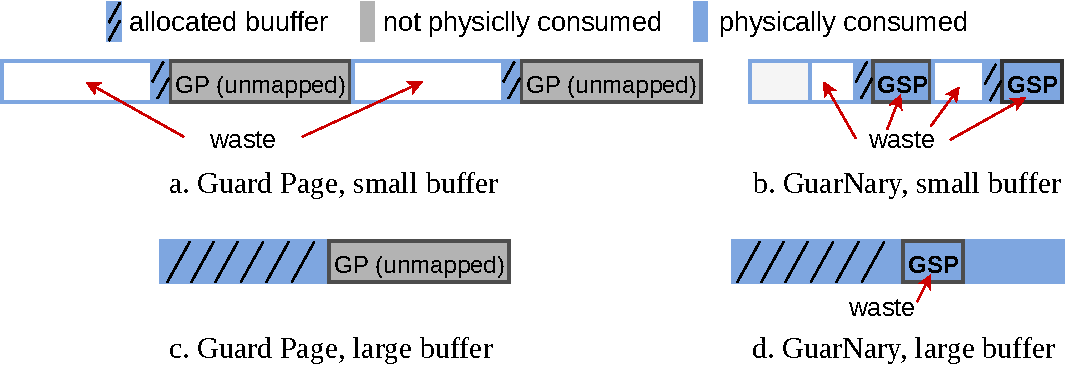
\includegraphics[width=.85\columnwidth]{figures/challenge1}
            Guarnary must satify the following equation: $\sum GN + \sum RGN < \sum RGP$
            \captionof{figure}{Challenge $C_1$ illustration. GSP stands for guarg sub-page, 
            $\sum GN$ memory consumed by guarnary, $\sum RGN$ and $\sum RGP$ internal fragmentation waste resp. of guarnary and guard page.}            
        \end{center}

        \vspace*{2mm}     

        \textcolor{blue}{\textbf{($C_2$) Costly hypercalls:}} SPP is configurable solely by the hypervisor.\\

        \textcolor{blue}{\textbf{($C_3$) Physical page heterogeneity:}} see Figure 4.\\

        \textcolor{blue}{\textbf{($C_4$) Protection pattern heterogeneity:}} the protection pattern is the bitmap of sub-pages that are write-protected within an SPP page.
        \begin{center}
            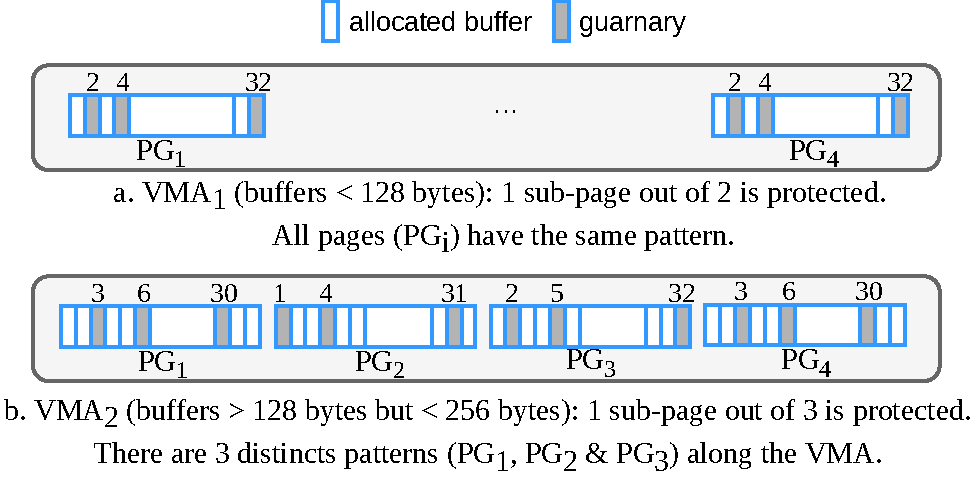
\includegraphics[width=.8\columnwidth]{figures/spp-pattern}
            \captionof{figure}{Protection pattern and frequency illustration.}            
        \end{center}

    \end{multicols}
}


%----------------------------------------------------------------------------------------
%	CONTACT INFORMATION
%----------------------------------------------------------------------------------------
\headerbox{Contact}{name=contact,column=3,aligned=references,above=bottom,boxColorOne=white}{ % This block is as tall as the references block

\begin{description}\compresslist
\item yves.kone@ens-lyon.fr
\item 
\item bitchebe@i3s.unice.fr
\item 
\item alain.tchana@ens-lyon.fr
\end{description}
}

%----------------------------------------------------------------------------------------
%	CONTRIB
%----------------------------------------------------------------------------------------


%----------------------------------------------------------------------------------------
%	PROBLEM
%----------------------------------------------------------------------------------------

% \headerbox{Probl\'ematique}{name=problem,column=1,below=spp,above=references}{ % This block's bottom aligns with the bottom of the conclusion block
% Le canari et la page de garde sont des solutions tr\'es utilis\'es et matures mais pr\'esentes cependant des inconv\'enients.
% \vspace{0.1cm}
% \newline
% \textbf{\textcolor{orange}{Le canari}}
% \begin{itemize}
% \vspace{-0.1cm}
%     \item \textbf{Surco\^ut m\'emoire raisonnable:} pour n buffer \`a prot\'eger, seulement n octets suppl\'ementaires sont n\'ecessaires.
%     \item \textbf{D\'etection peu efficace:} la d\'etection de d\'epassements est \textcolor{orange}{\textbf{asynchrone}} et \`a se fait au niveau logiciel.
% \end{itemize}
% \textbf{\textcolor{orange}{La page de garde}}
% \begin{itemize}
%     \vspace{-0.1cm}
%     \item \textbf{D\'etection synchrone:} elle se fait lors de la traduction d'adresse.
%     \item \textbf{Surco\^ut m\'emoire potentiellement tr\`es \'elev\'e:} pour prot\'eger N buffer il faut au minumum \textcolor{orange}{\textbf{N pages}}.
% \end{itemize}
% \begin{figure}[H]
%     \centering
%     \vspace{-0.6cm}
%     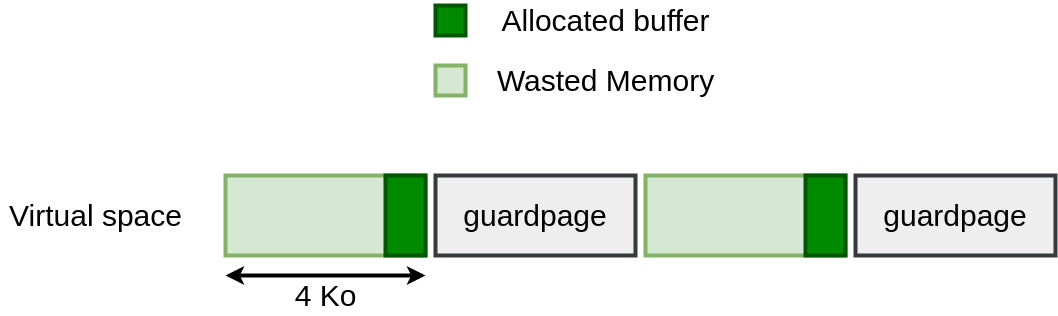
\includegraphics[width=0.9\linewidth]{guardpage_wasted}
%     \captionof{figure}{Sch\'ema de buffers prot\'eg\'es par des pages de garde. 
%     On voit ici que la m\'emoire consomm\'ee est de 8Ko (2 pages).}
% \end{figure}
% }

%----------------------------------------------------------------------------------------
%	MOTIV
%----------------------------------------------------------------------------------------

\headerbox{3. Intel SPP: Sub-Page Write Permission}{name=results2,column=0,below=ctxmotiv,above=references, span=2}
{ % This block's bottom aligns with the bottom of the conclusion block
    SPP~\cite{spp} is a recent Intel hardware virtualization feature that allows the hypervisor to write-protect guest’s memory at a sub-page (128B) granularity instead of 4KB.
    \begin{center}
        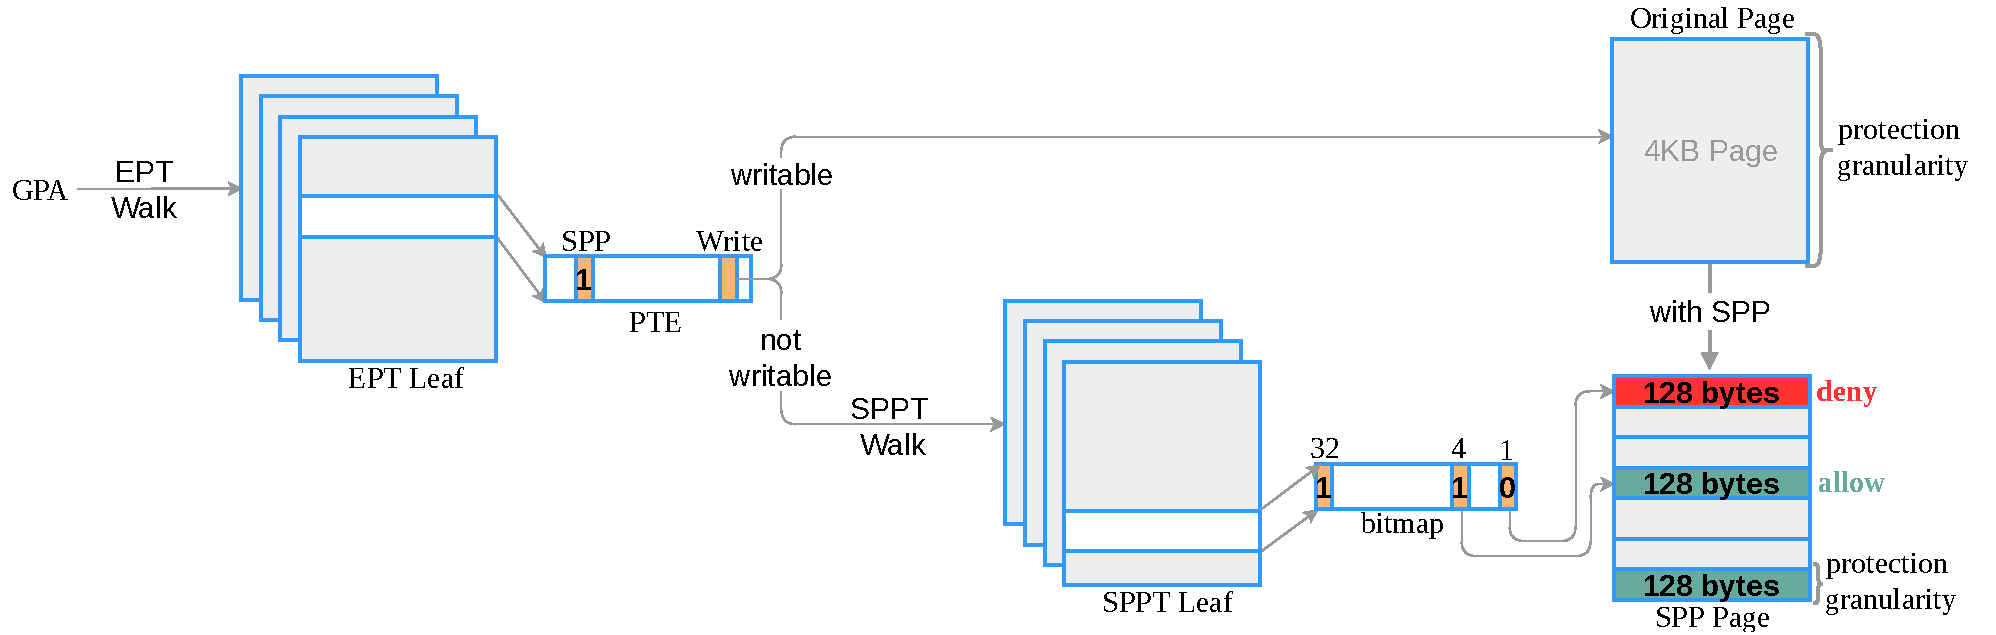
\includegraphics[width=.95\columnwidth]{figures/spp_walk}
        \captionof{figure}{Overview of SPP functioning.}        
    \end{center}    
}

%----------------------------------------------------------------------------------------

\end{poster}

\end{document}